\section{TCP/NC的实现}
%%数据包编码
\subsection{数据包编码}
%%有限域
\begin{frame}[t]
	\frametitle{有限域}
	\vspace{-1em}
	\begin{block}{有限域}
		有限域提供了一个有限集,
		在该有限集上明确定义且有效地实现了加法、减法、乘法和除法运算,
		并允许系统使用矩阵、行列式、高斯消元等线性代数中常见的运算工具来解决该域上的联立线性方程组问题。
	\end{block}
	\begin{columns}
		%%第一列
		\begin{column}{0.5\textwidth}
			\begin{table}[htp]
				\centering
				\label{tab:youxianyujia}
				\begin{tabular}{l|llll}
					\toprule
					+&0&1&A&B\cr
					\midrule
					0&0&1&A&B\cr
					1&1&0&A&B\cr
					A&A&B&0&1\cr
					B&B&A&1&0\cr
					\bottomrule
				\end{tabular}
			\end{table}
		\end{column}
		%%第二列
		\begin{column}{0.5\textwidth}
			\begin{table}[htp]
				\centering
				\label{tab:youxianyucheng}
				\begin{tabular}{l|llll}
					\toprule
					$\cdot$ &0&1&A&B\cr
					\midrule
					0&0&0&0&0\cr
					1&0&1&A&B\cr
					A&0&A&B&1\cr
					B&0&B&1&A\cr
					\bottomrule
				\end{tabular}
			\end{table}
		\end{column}
	\end{columns}
	\note{
		TCP/NC中需要对数据包进行编码,
		而从TCP层下到NC层的数据包都是字节流。
		如何抽象出前面谈到的报文概念?如何对数据包进行各种操作,如加减乘除?
		有限域为我门提供了一个数学工具。
	}
\end{frame}
%%编码示例
\begin{frame}
	\frametitle{编码示例}
%	我们以两个数据包$p_{1}$和$p_{2}$的运算为例,
%	说明如何对数据包进行编码。
	假定数据包$p_{1}$和$p_{2}$都为一个2字节的报文,
	以比特流的形式表示,
	$p_{1}=\{1010\ 0101\ 0110\ 1111\}$,$p_{2}=\{1111\ 0000\ 1101\ 0110\}$,
	我们需要计算$p_{encoded}=7p_{1} \oplus 13p_{2}$的值。
	步骤如下:
	\begin{enumerate}[(1)]
		\item 取$p_{1}$和$p_{2}$的第一个字节,
		分别是$\{1010\ 0101\}$和$\{1111\ 0000\}$,
		对应的十进制为$D_{p_1}=165$和$D_{p_2}=240$。
		在有限域$GF(2^8)$下计算$7\times 165$和$13 \times 240$的值,
		分别是$0xc6$和$0xc4$。
		则$p_{encoded}$的第一个字节为$0xc4 \oplus 0xc6=0x02$,
		二进制表示为$\{0000\ 0010\}$。
		\item 同样的方法处理$p_{1}$和$p_{2}$的第二个字节,
		结果为$\{1010\ 0111\}$。
		\item 拼接两个结果得到$p_{encoded}=\{0000\ 0010\ 1010\ 0111\}$。
	\end{enumerate}
\end{frame}
\subsection{技术路线}
%%设备选型
\begin{frame}
	\frametitle{设备选型}
	\begin{columns}
		\begin{column}{0.4\textwidth}
			考虑到无人机视频传输的应用场景,
			及TCP/NC需要参与到网络协议栈的流程中去,
			选用Raspberry Pi这款基于Linux的嵌入式设备,
			部署TCP/NC协议,如图\ref{fig:rasp}所示。

		\end{column}
		\begin{column}{0.5\textwidth}
			\begin{figure}
				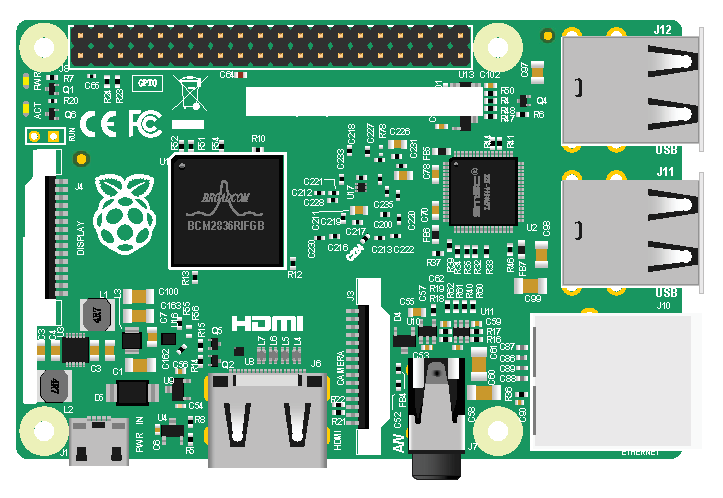
\includegraphics[height=4cm]{figures/rasp.eps}
				\caption{Raspberry Pi板子}
				\label{fig:rasp}
			\end{figure}
		\end{column}
	\end{columns}
	\note{
		Raspberry Pi是一款ARM架构的单板机,
		板载了以太网卡。支持CSI接口,
		方便外接摄像头,进行后期无人机视频传输测试。
		操作系统选择树莓派基金会的Debian系统,
		内核版本为3.18。
	}
\end{frame}
%%Netfilter
\begin{frame}
	\frametitle{Netfilter}
	\begin{columns}
		\begin{column}{0.5\textwidth}
			NC层实施方案有两种:
			\begin{enumerate}
				\item 直接在内核的TCP协议源码上更改,添加NC层的各个模块,然后再编译内核源码
				\item 利用Linux内核提供给用户用于处理网络封包的框架——Netfilter。
			\end{enumerate}
			本文将TCP/NC部署在Netfilter的NF\_IP\_LOCAL\_IN和NF\_IP\_LOCAL\_OUT处。
		\end{column}
		\begin{column}{0.4\textwidth}
			\vspace{-1.5em}
			\begin{figure}
				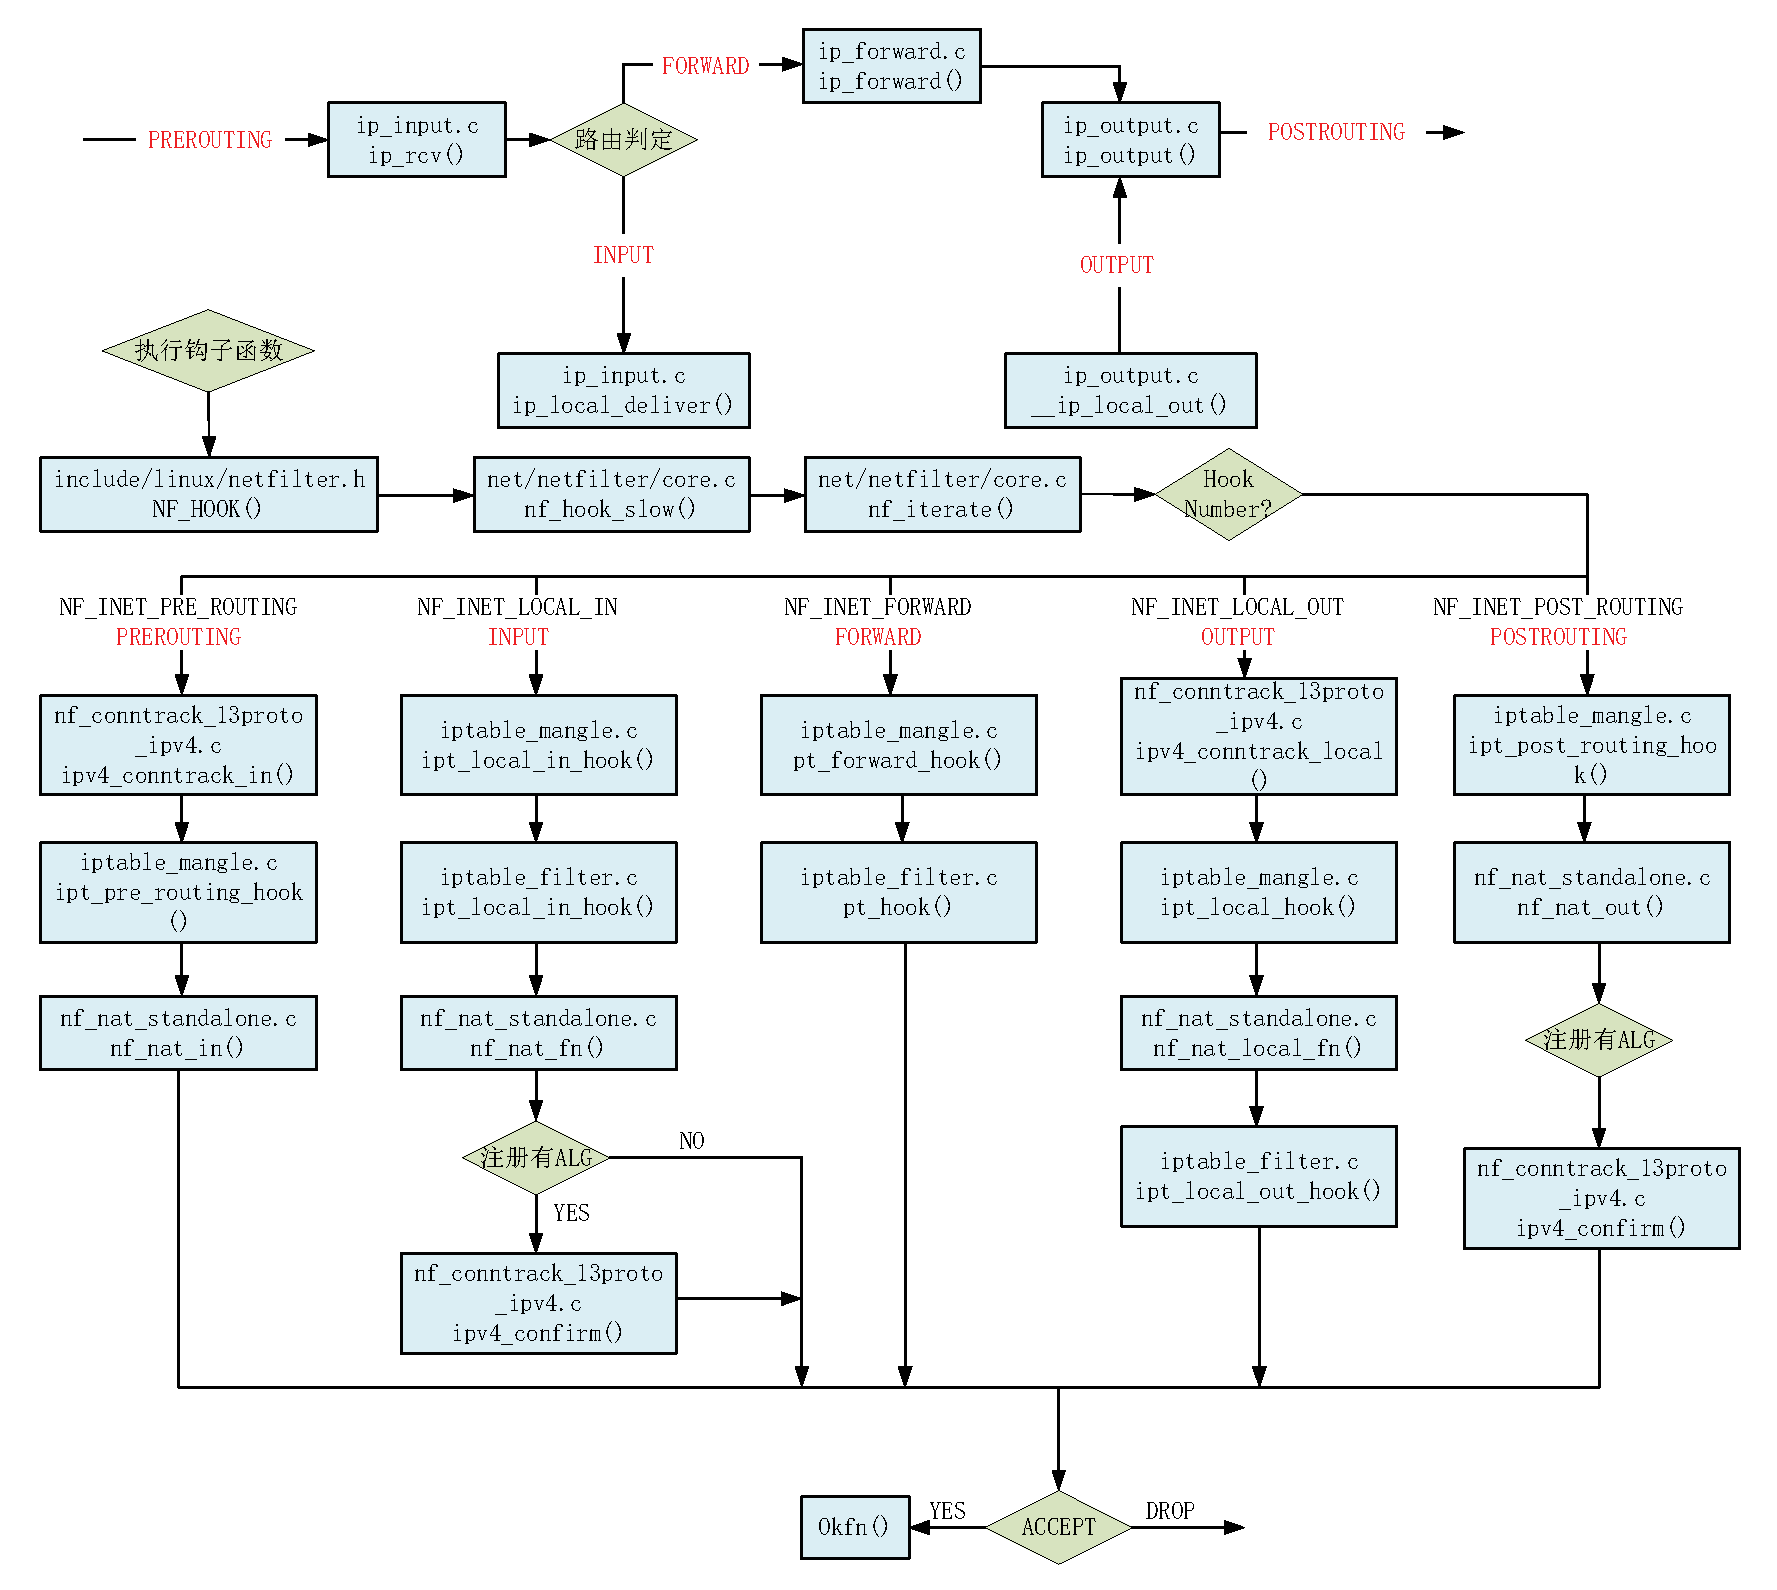
\includegraphics[height=5cm]{../figures/packetflow.eps}
				\caption{Netfilter及其在内核源码中调用关系}
				\label{fig:packetflow}
			\end{figure}
		\end{column}
	\end{columns}

	\note{
	}
\end{frame}
%%关键数据结构
\begin{frame}
	\frametitle{关键数据结构}
	NC层在NF\_IP\_LOCAL\_IN和NF\_IP\_LOCAL\_OUT这两个钩子点获得的都是单独的报文,
	其形式为\emph{sk\_buff}结构体,如图\ref{fig:skbuff}所示。
		\begin{columns}
		\begin{column}{0.5\textwidth}
			数据包在Linux的网络协议栈的不同层之间传递,
			其体现形式就是不同层的函数对一个数据包对应的\emph{sk\_buff}进行各种操作。
			\\
			TCP/NC通过\emph{sk\_buff}获得数据包的字节流,
			然后对数据包进行编码。
		\end{column}
		\begin{column}{0.4\textwidth}
			\vspace{-2em}
			\begin{figure}
				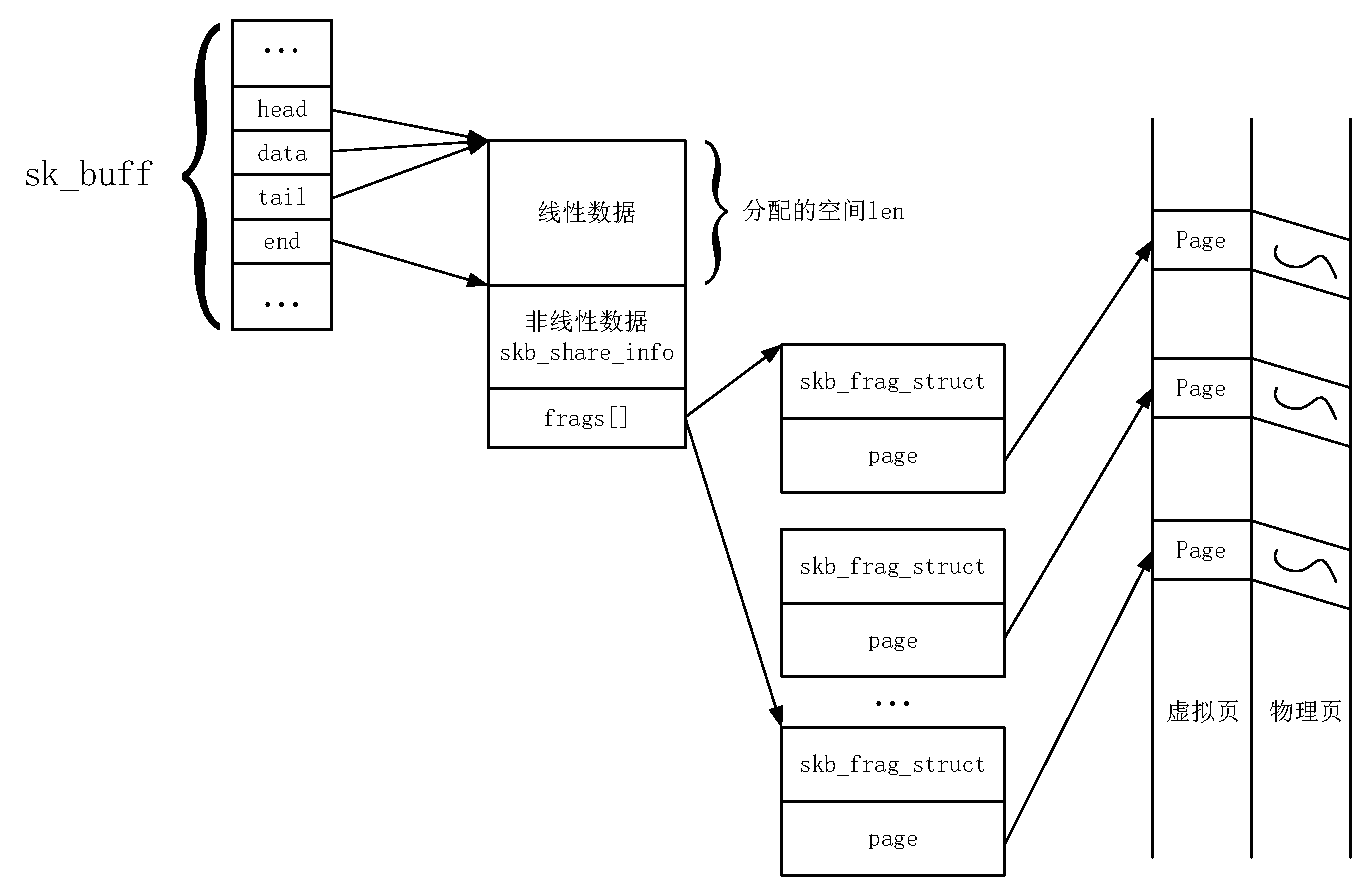
\includegraphics[height=4cm]{../figures/skbuff.eps}
				\caption{skbuff结构}
				\label{fig:skbuff}
			\end{figure}
		\end{column}
	\end{columns}
	
\end{frame}
\subsection{NC层关键技术}

%%NC层总体框架
\begin{frame}[t]
	\frametitle{NC层总体框架}
	\begin{columns}[t]
		\begin{column}{0.4\textwidth}
		图\ref{fig:jiagou}为NC层总体框架。
		虚线框内的即为网络编码层。
		\end{column}
		\begin{column}{0.5\textwidth}
			\vspace{-2.5em}
			\begin{figure}
				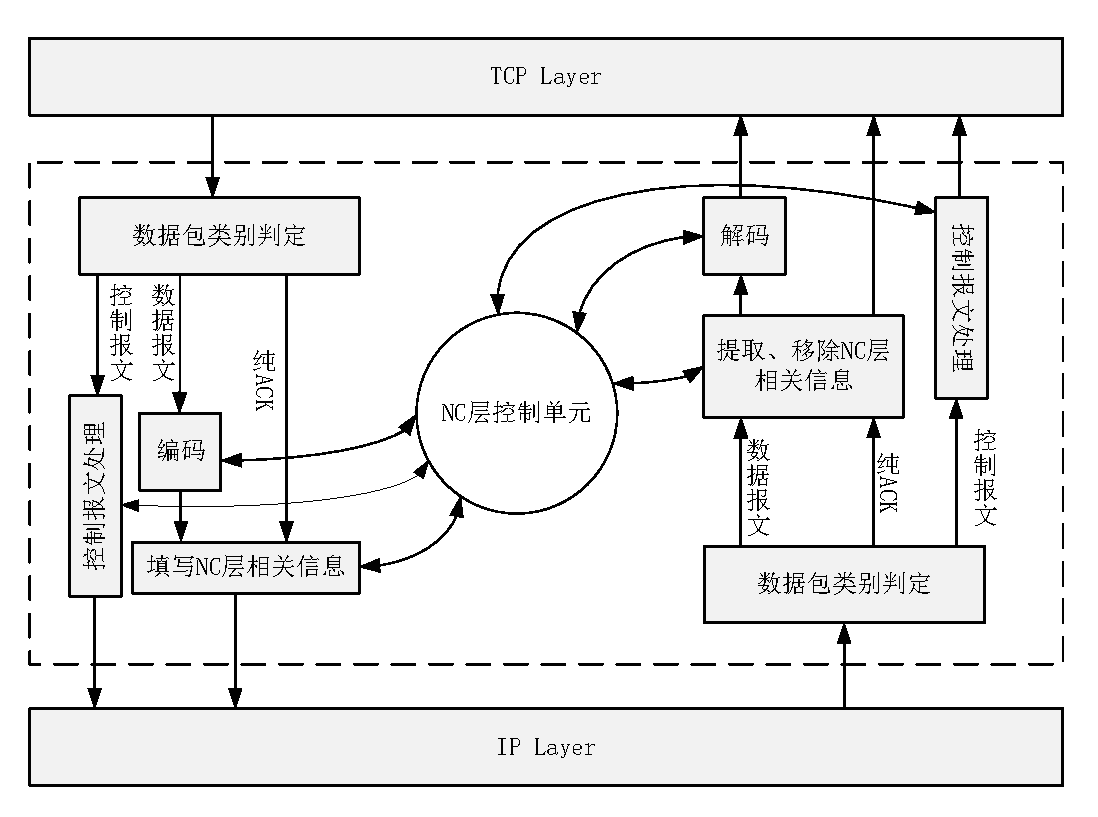
\includegraphics[height=5cm]{../figures/jiagou.eps}
				\caption{NC层总体框架}
				\label{fig:jiagou}
			\end{figure}
		\end{column}
	\end{columns}
\end{frame}
%%NC层头部
\begin{frame}
	\frametitle{NC层头部}
	\begin{columns}
		\begin{column}{0.4\textwidth}
			发送端需要给产生的编码包添加NC头部,
			其中包含编码系数等信息,接收端利用这些信息进行解码。
			图\ref{fig:codingheader}为NC报文的头部。
		\end{column}
		\begin{column}{0.6\textwidth}
			\begin{figure}
				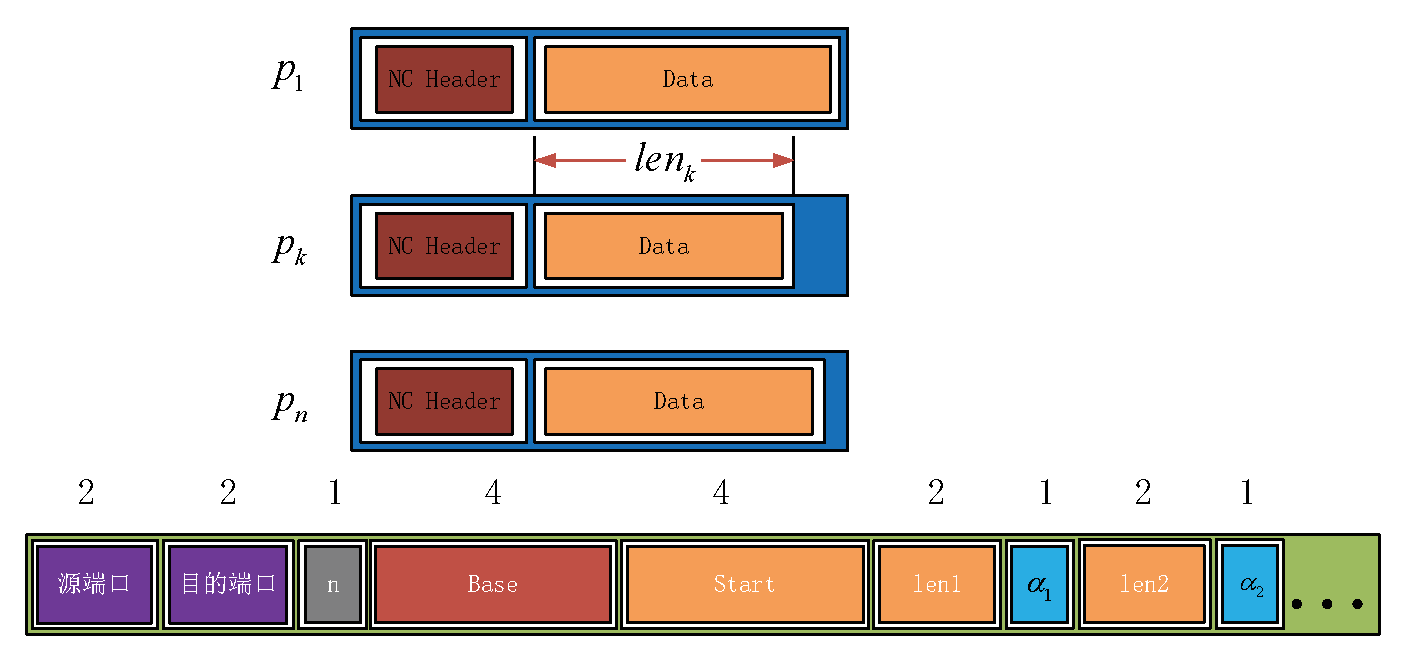
\includegraphics[height=4cm]{../figures/codingheader.eps}
				\caption{NC层头部}
				\label{fig:codingheader}
			\end{figure}
		\end{column}
	\end{columns}
	\note{
	}
\end{frame}
%%编码端
\begin{frame}
	\frametitle{编码}
	\begin{columns}
		\begin{column}{0.4\textwidth}
			发送端的NC层维护了一个\emph{sk\_buff}的链表\emph{sk\_buff\_head},
			存放从TCP层下来的数据包。
			此链表也作为发送端的编码缓存,
			其插入操作发生于有数据包文从TCP层下来时;
			删除操作发生于收到接收端的NC层的ACK报文时。
			编解码步骤如右图。
		\end{column}
		\begin{column}{0.6\textwidth}
			\vspace{-2.5em}
			\begin{figure}
				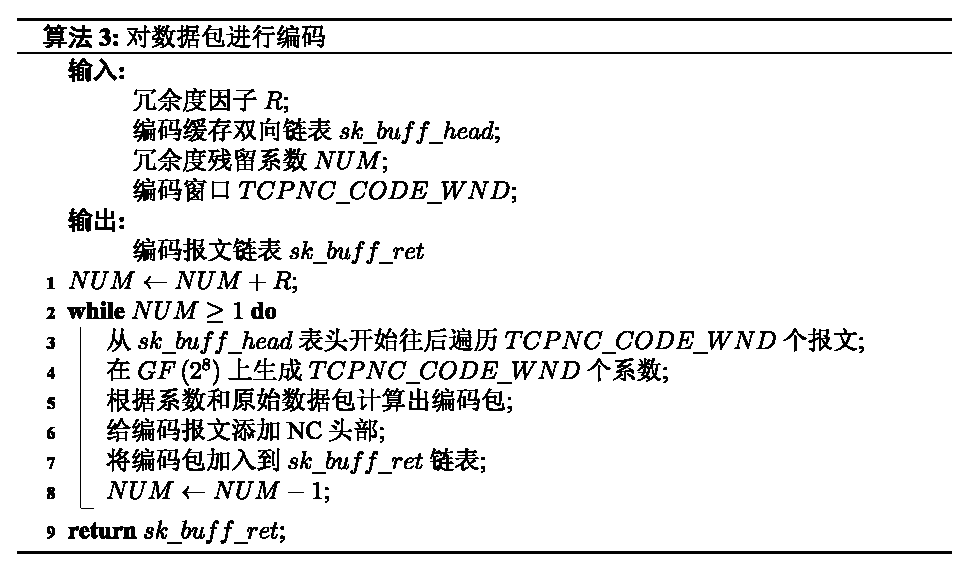
\includegraphics[height=5.5cm]{figures/encoding.eps}
			\end{figure}
		\end{column}
	\end{columns}
\end{frame}

%%解码
\begin{frame}
	\frametitle{解码}
	解码步骤如下:
	\begin{enumerate}
		\item 提取编码报文的编码系数
		\item 对系数进行高斯消元
		\item 利用高斯消元的结果对数据包报文部分进行相应的操作
	\end{enumerate}
	\begin{block}{解码关键技术}
		\begin{enumerate}
			\item \emph{backlog队列},接收端收到的编码数据包首先都会进入\emph{backlog}队列
			\item \emph{decoding队列},\emph{decoding}队列的数据包为目前在解码矩阵中的数据包,可能参与到对数据包的解码操作
			\item \emph{decoded队列},\emph{decoded}队列存放的是目前已经解码出的数据报文。
		\end{enumerate}
	\end{block}
\end{frame}

%%接收窗口
\begin{frame}
	\frametitle{接收窗口}
	考虑到NC层提前确认了一些数据包,
	在接收端,我们需要对发出去的ACK报文的接收窗口值作出修改。
	\begin{figure}
		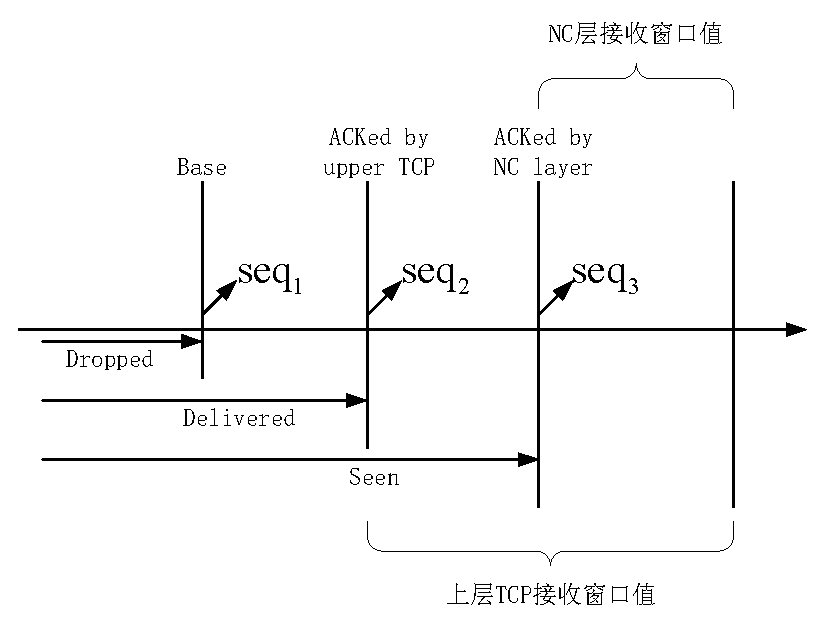
\includegraphics[height=4cm]{../figures/rcvwnd.eps}
		\label{fig:rcvwnd}
		\caption{接收窗口设定}
	\end{figure}
\end{frame}

\subsection{测试结果和结论}
\begin{frame}[allowframebreaks]
	\frametitle{测试}
	\begin{columns}
		\begin{column}{0.4\textwidth}
			\begin{figure}
				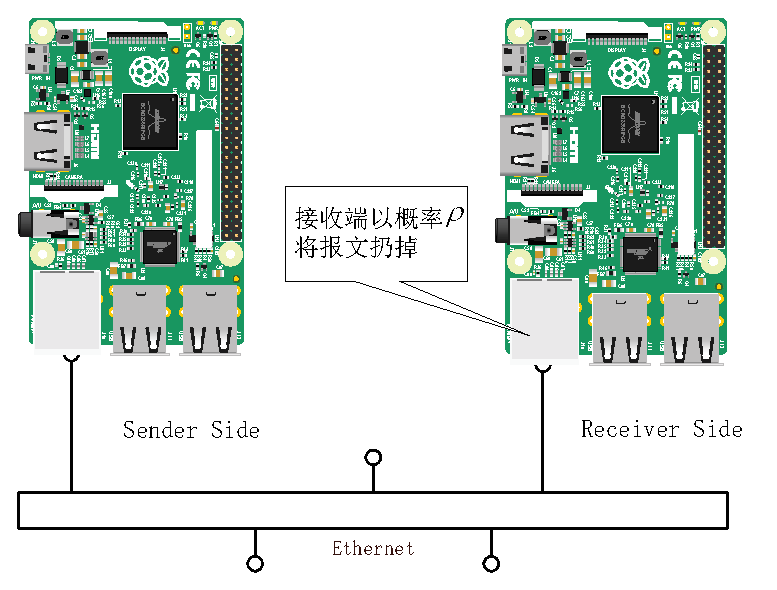
\includegraphics[height=4cm]{../figures/tuopu.eps}
				\label{fig:tuopu}
				\caption{测试拓扑}
			\end{figure}
		\end{column}
		\begin{column}{0.6\textwidth}
			\vspace{-1.5em}
			\begin{table}[htp]
				\centering
				\small
				\caption{测试环境参数}
				\label{tab:ceshicanshu}
				\begin{tabular}{ll}
					\toprule
					参数名称&参数值\tabularnewline
					\midrule
					机型		&Raspberry Pi 2 Model B\tabularnewline
					CPU		&900MHz Cortex-A7\tabularnewline
					RAM			&1G\tabularnewline
					以太网卡 	&10M/100M\tabularnewline
					操作系统 &Debian\tabularnewline
					内核版本 &Linux 3.18\tabularnewline
					TCP协议版本 &TCP-Reno\tabularnewline
					测试工具 &iperf\tabularnewline
					测试时间 &60秒\tabularnewline
					\bottomrule
				\end{tabular}
			\end{table}
		\end{column}
	\end{columns}
	\newpage
	固定链路丢包率为$5\%$,
	测试冗余度对吞吐率的影响如图\ref{fig:throughput2redundancy}。
	
	我们对不同丢包率下TCP和TCP/NC的性能进行了对比测试,
	如图\ref{fig:throughput2loss}所示,
	其中TCP/NC的吞吐率都为最优吞吐率。
	\begin{columns}
		\begin{column}{0.5\textwidth}
			\begin{figure}
				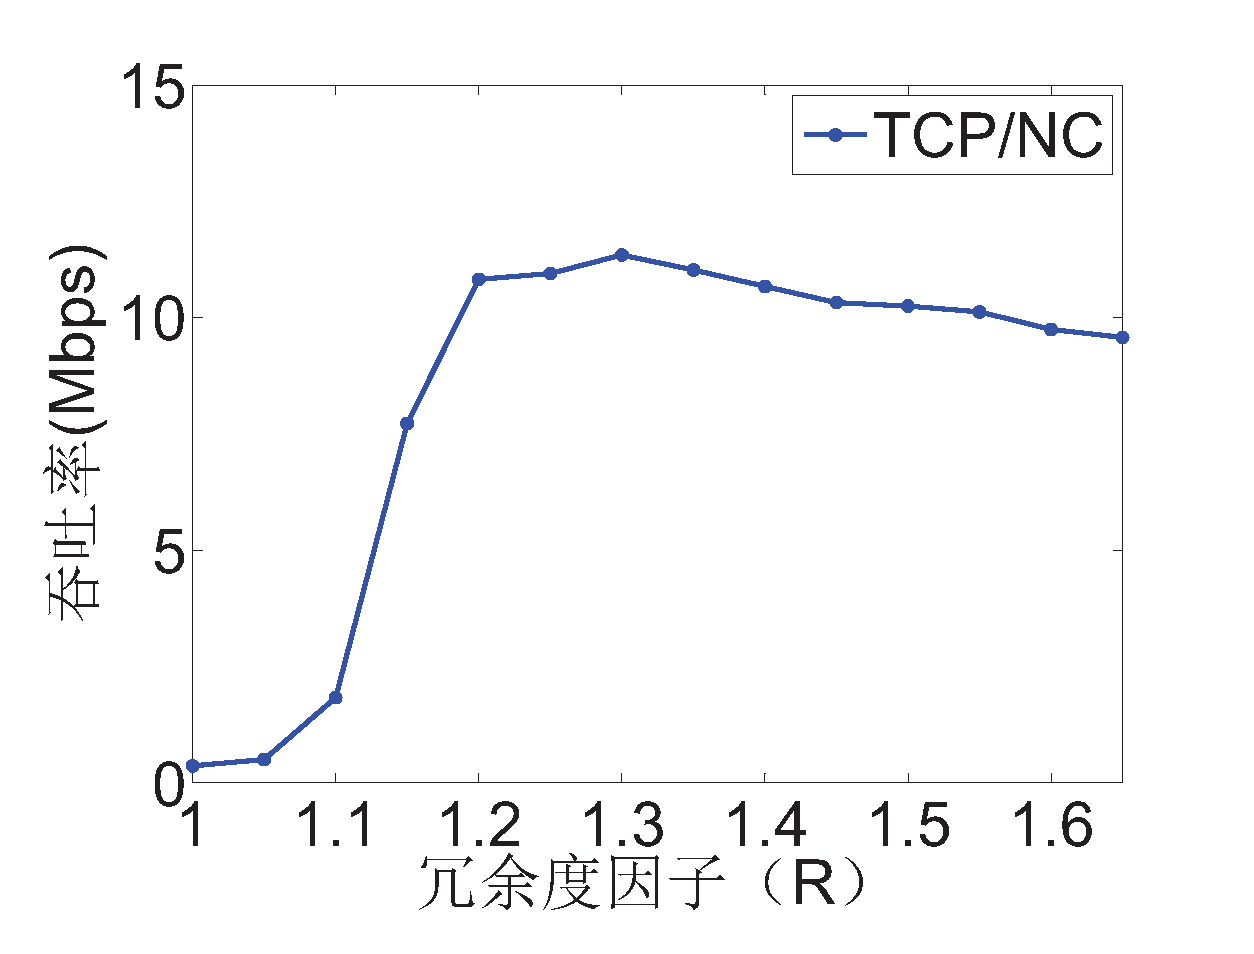
\includegraphics[height=3.5cm]{../figures/redundancy.eps}
				\caption{吞吐率-冗余度}
				\label{fig:throughput2redundancy}
			\end{figure}
		\end{column}
		\begin{column}{0.5\textwidth}
			\begin{figure}
				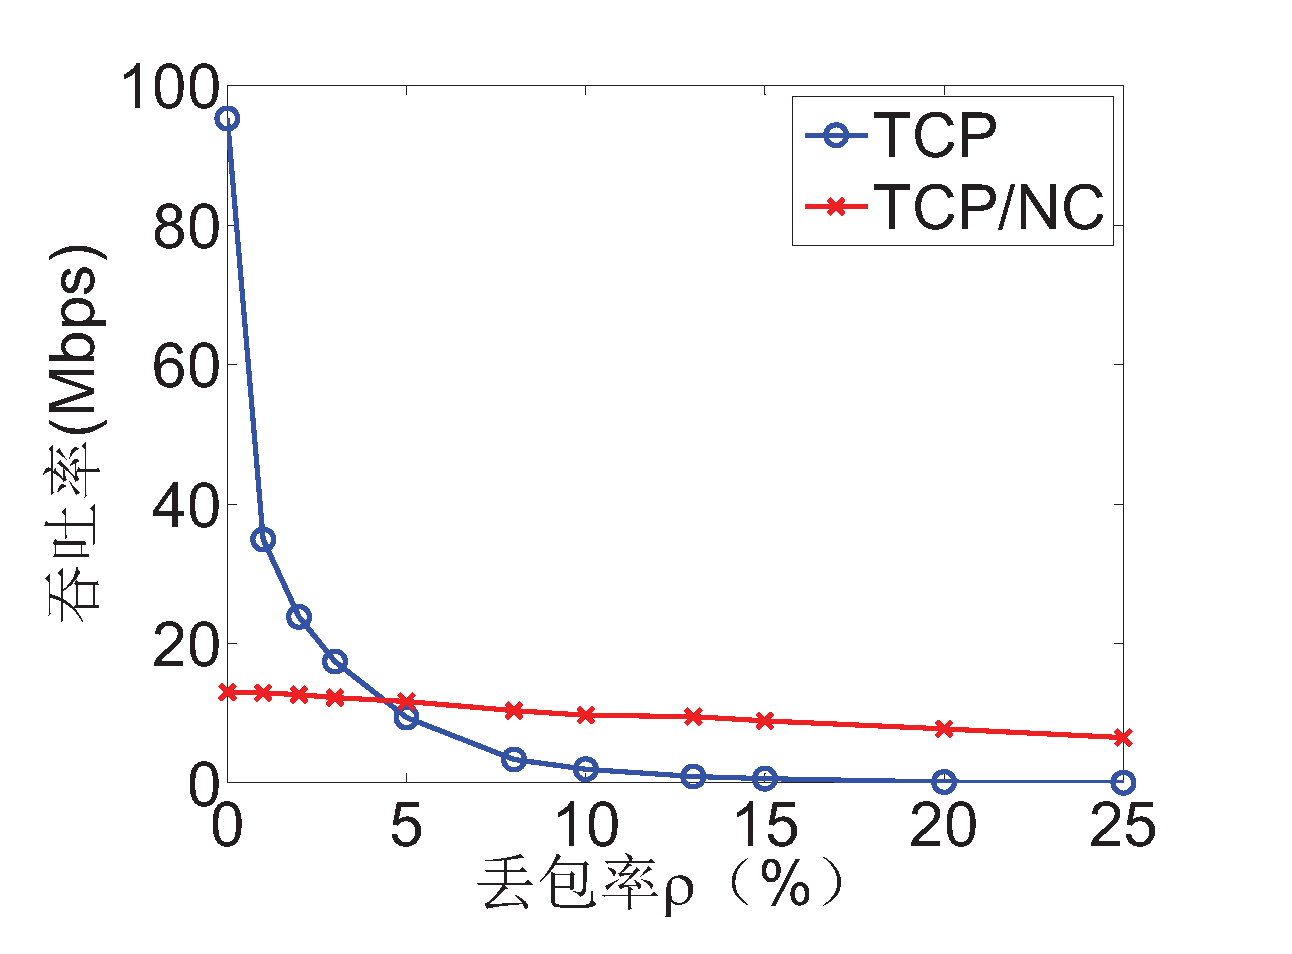
\includegraphics[height=3.5cm]{../figures/throughput2lossrate.eps}
				\caption{吞吐率-丢包率}
				\label{fig:throughput2loss}
			\end{figure}
		\end{column}
	\end{columns}
\end{frame}

%\begin{frame}
%	\frametitle{结论}
%\end{frame}















